\documentclass[10pt,twocolumn,letterpaper]{article}

\usepackage{cvpr}
\usepackage{times}
\usepackage{epsfig}
\usepackage{graphicx}
\usepackage{amsmath}
\usepackage{amssymb}

% Include other packages here, before hyperref.

% If you comment hyperref and then uncomment it, you should delete
% egpaper.aux before re-running latex.  (Or just hit 'q' on the first latex
% run, let it finish, and you should be clear).
\usepackage[breaklinks=true,bookmarks=false]{hyperref}

\cvprfinalcopy % *** Uncomment this line for the final submission

\def\cvprPaperID{****} % *** Enter the CVPR Paper ID here
\def\httilde{\mbox{\tt\raisebox{-.5ex}{\symbol{126}}}}

% Pages are numbered in submission mode, and unnumbered in camera-ready
%\ifcvprfinal\pagestyle{empty}\fi
\setcounter{page}{1}
\begin{document}

%%%%%%%%% TITLE
\title{Recognizing Ancient Greek Handwriting Using Modern Training Data}

\author{Sean Karlage\\
University of Kentucky\\
Lexington, KY\\
{\tt\small sean.karlage@uky.edu}
}
% For a paper whose authors are all at the same institution,
% omit the following lines up until the closing ``}''.
% Additional authors and addresses can be added with ``\and'',
% just like the second author.
% To save space, use either the email address or home page, not both

\maketitle
%\thispagestyle{empty}

\section{Progress}
\begin{itemize}
    \item Complete changed my project around after realizing that it was not feasible to use off-the-shelf OCR scanners to try and recognize handwritten text
    \item At the recommendation of Dr. Seales, dropped the notion of scanning my own papyrus on the scanner in Marksbury because it would take too long to complete and "the scanner is really finicky"
    \item Iterated through several project ideas until I was able to come up with the current idea
    \item Did some initial research and tried to locate datasets. Found the GCDB database of handwritten characters. I would like to evaluate classifiers that have been trained with this data to detect those from ancient Greek writings from http://sites.lib.byu.edu/scholarsarchive/byu-multi-spectral-imaging-project/
    \item Using OpenCV + Python, built a simple kNN classifier that was trained and evaluated on the GCDB data, obtaining 66.8\% accuracy in recognition
\end{itemize}

\section{Issues}
\begin{itemize}
    \item Still do not have manually-segmented letterforms from BYU corpora, but expect to have them in the coming weeks with the help of Scrolls research team members. This is the key part of the project
    \item Need to create more classifiers using different ML techniques to try and get the best detector possible
    \item Need to determine which features would be the best for testing on modern Greek handwriting and then evaluating on ancient Greek
\end{itemize}

%%%%%%%%% ABSTRACT
\begin{abstract}
    While recognition of machine-printed text with automated procedures is considered a solved problem by most computer scientists, recognition of handwriting is still a difficult problem in the field of text recognition. On top of these difficulties, recognition of ancient manuscript letterforms is even more difficult due to document deformities and letterform occlusion. Because of the lack of datasets for ancient Greek handwriting, classifiers employing a variety of machine learning techniques were trained on the [GCBD] dataset and evaluated on both samples from that dataset and on manually-segmented letterforms from an ancient Greek manuscript corpus.
\end{abstract}

%%%%%%%%% BODY TEXT
\section{Introduction}

Automated recognition of machine-printed text is generally considered by some to be a solved problem in the field of computer vision. Many commercial and open-source systems exist that are designed to take as input images or scans of machine-printed text and output corresponding text elements with a high degree of accuracy. However, this automated process is much more difficult when it comes to recognizing handwritten text for a variety of reasons: different writing styles, various font embellishments, irregular line widths, etc.

Recognition of ancient handwritten text, in particular, represents a unique challenge in this field; in addition to the above-mentioned problems, texts can be malformed, occluded by foreign material on the document, or simply have degraded due to age. The ability to automatically recognize such text would be a real boon for document researchers, as not only would they be able to more easily interpret ancient text, but also contribute to the digital archival of said text.

%-------------------------------------------------------------------------
\subsection{Motivation}

As a part of the larger “volume cartography” project occurring at [VisCenter], a need arose for automated recognition of ancient Greek handwritten letterforms.  Because of the volume of data that could potentially contain text is large, manually parsing flattened, textured volume data for possible letterforms is infeasible. Furthermore, in addition to team member validation, professional analysis from experts in ancient Greek writings would be required in order to evaluate and validate any potential discoveries.

As a first pass, however, automated recognition of potential letterforms provides a good estimate of signal-to-noise ratio and evaluation of letterform extraction procedures. To the author’s knowledge, however, no open or commercial database of segmented ancient Greek handwritten letterforms exists with which to serve as a training dataset for any potential text classifier. Instead, the author proposes to train classifiers based on datasets of modern Greek handwriting - in particular, the dataset proposed in [GCDB] - and evaluate based on hand-labeled text from the document collection of [BYU].

%------------------------------------------------------------------------
\section{Related Work}

Automated recognition of Early Christian Greek manuscripts has been carried out previously by [CIL], in which the authors employed a segmentation-free approach by detecting open and closed cavities in letterforms and using those as a basis with which to extract features of each character. The system developed by the authors obtained a recall value of 89\% for simple letterforms in their testing dataset.
\begin{itemize}
    \item The database of letterforms used by the authors is not available for further study to the best of my knowledge. I have contacted one of the authors and am waiting to hear back
\end{itemize}

[HisDoc] project involved not only handwriting recognition and digitization of manuscript text data, but also developing an information retrieval system around recovered data. The authors developed this system and applied it primarily to three text corpora in different languages (Latin, German, and English, respectively). Their system accurately segmented and recognized text from each corpus and, using a neural network-based approach, had word recognition rates of less than 10\%.

[Diem1], [Diem2] proposed a binarization-free approach to recognizing letterforms from ancient Slavonic documents using SIFT features, SVM classifiers, and finally a weighted voting algorithm based on pre-classified local descriptors. Not applying binarization filters to input documents allowed for more data from each letterform, particularly those that were heavily degraded or experienced occlusion from stains or tears in the manuscript.

The authors of [GRUHD] were the first to develop an open dataset of modern Greek handwriting that contained extensive metadata about participants, as well as providing very well-segmented letterforms and words from each individual author. The sample text contains simple Greek words as well as both uppercase and lowercase Greek letters and numerals from 1000 individual contributors. This database has been supplanted by [GCDB], from the same authors, with improvements to database architecture and archival. GCDB also contains Greek word samples and letterforms from 305 unique contributors.

%-------------------------------------------------------------------------
\section{Problem Statement}

With the lack of ancient Greek handwriting dataset availability, building and evaluating a detector on live data proves difficult. In order to approximate a recognition system, we propose to answer the following primary research question:

\begin{quote}
    \textit{Can a handwriting recognition system that is trained on modern Greek handwriting be used to classify segmented letterforms from ancient Greek manuscripts?}
\end{quote}

A variety of classifiers will be built that will be validated against both the training dataset as well as live data from the corpora of [BYU].

%-------------------------------------------------------------------------
\section{Approach}

In order to get a variety of results from training data, a host of classifiers will be developed using a variety of common learning algorithms. A fraction of the dataset from [GCDB] will be used to train each classifier, and the remaining samples will comprise the testing/evaluation dataset. Each trained classifier will also be evaluated on individual letterforms extracted from the corpora of [BYU].

%-------------------------------------------------------------------------
\subsection{k-Nearest Neighbors}

A very simple k-Nearest Neighbors classifier was developed using Python and OpenCV. The built-in kNN classifier in OpenCV was used as the base, and was trained on 50\% of the GCDB dataset. The remaining half of the data served as evaluation data.
\begin{itemize}
    \item As I try more classifiers, I will put them in subsections below this one
    \item Once I get the extracted letterforms from the BYU corpora, I will go back and evaluate the trained kNN classifier on those letterforms and report the results in the appropriate section
    \item Also want to try out other features such as Zernicke moments from [Kale]
\end{itemize}

%-------------------------------------------------------------------------
\section{Evaluation}
\subsection{k-Nearest Neighbors}

The simple k-Nearest Neighbors classifier was evaluated on the GCDB dataset, with 50\% of the dataset comprising the training data, and the other 50\% comprising the evaluation data. The classifier was run for differing values of $k$ in the range [1, 20]. The plot of accuracy vs. values of $k$ are shown in Figure 1.

\begin{figure}
    \begin{center}
        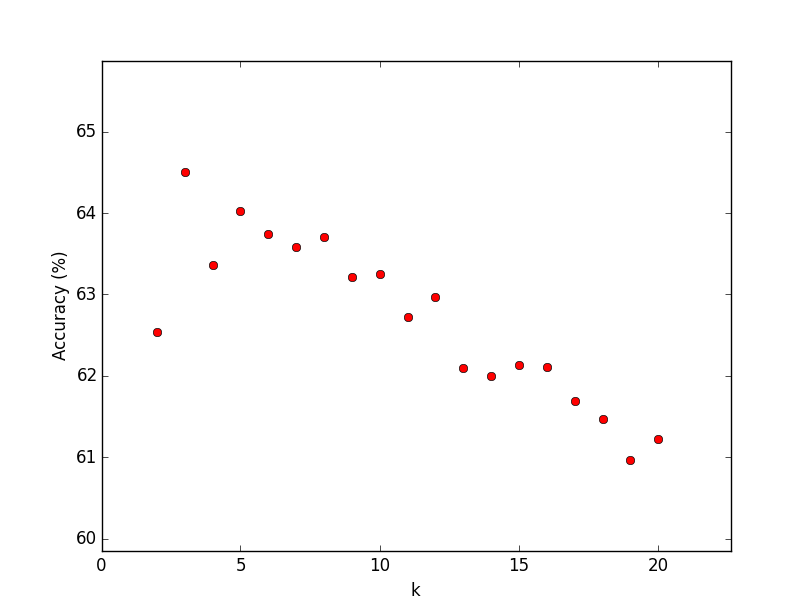
\includegraphics[width=0.8\linewidth]{res/figure_1.png}
        \caption{Plot of k-Nearest Neighbors accuracy vs. increasing values of $k$}
    \end{center}
\end{figure}

\begin{itemize}
    \item Would like to have a color plot of the clusters in the future here as well
    \item As I add more classifiers, I will expand this section in tandem with the above \textit{Approach} section
\end{itemize}

%-------------------------------------------------------------------------
\section{Discussion}

\begin{itemize}
    \item Trained kNN classifier on GCDM dataset, achieved maximum accuracy of 66.8\% recognition
    \item Will list more summary results for each classifier
    \item Once I get evaluation data from BYU corpora, will compare results and determine whether this approach is viable or not
\end{itemize}

%-------------------------------------------------------------------------
\section{References}

{\small
\bibliographystyle{ieee}
\bibliography{egbib}
}

\end{document}
